\section{Results}
\label{results}

Borrowing again from Flaxman 2014, the models were evaluated on a variant of $R^2$ that captures the reduction in total variance from each kernel component, which in turn can be interpreted as a measure of what components are most important in explaining the model. The error from predicting solely on the prior spatial expectation $e_s$ serves as a baseline for comparison:

$$ 1 - \frac{\sigma_{s,t}(n_{s,t}- \hat{n_{s,t}})^2}{\sigma_{s,t}(n_{s,t} - e_{s})^2}$$

Mean Squared Error (MSE) was also calculated for each the predictions from each $f_i(s,t)$ and compared to an AR(1) model that only relies on temporal predictions from the prior period.


\subsection{Long Term Predictions}

 Weekly traffic collision and injury data was aggregated to the level of New York City neighborhoods for this set of experiments. While data is available for the past five years, there appears to have been a reporting error for part of 2016 which made the year of data problematic for both model fitting and testing. It would have been ideal to fit the model based on multiple years of data leading up to the latest available data, but given the unreliable data the best alternative was fitting the LGCP on three years of data from July 2012 to July 2015, and leaving the following 52 weeks for out-of-sample prediction. The prior spatial expectation $e_s$ was taken from New York State Department of Health statistics for injuries stemming from motor vehicle collisions during the in-sample period \cite{nys_crash_stats}. \par

 \todo{chart of data errors}


 \begin{figure}[h!]
   \caption{A Gaussian Process fit to weekly pedestrian injuries in New York City from 2012 to 2015. The dotted line shows where out of sample prediction begins.}
   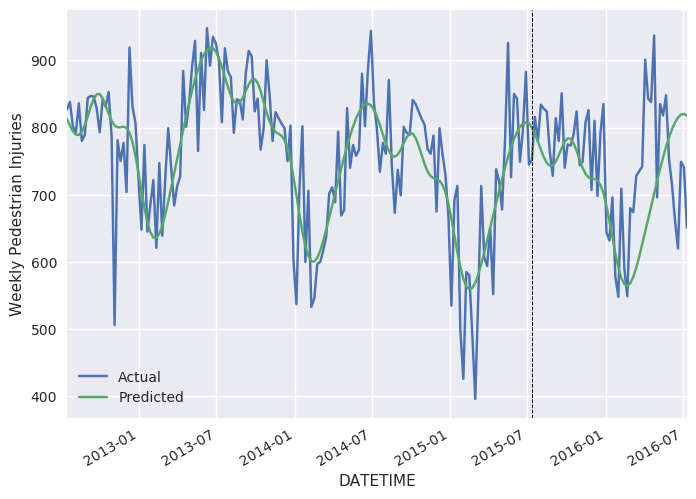
\includegraphics[width=0.5\textwidth]{citywide_predictions}
 \end{figure}

\todo{discussion of confidence?}

Since the kernel components are all additive they can provide an interpretable decomposition of the model components. There is clear annual periodicity in the model, which is also confirmed by the period parameter fitted being almost exactly 52. The linear kernel component also suggests a small downward long-term trend in pedestrian injuries.

\begin{table}[]
\centering
\caption{My caption}
\label{citywide_parameters}
\begin{tabular}{lll}
                                      & prior                                   & value \\
PartialVGP/kern/periodic/period       & None                                    & 0.52 \\
PartialVGP/kern/periodic/variance     & student-T({[} 0.{]},{[} 1.{]}{[} 4.{]}) & 0.03  \\
PartialVGP/kern/periodic/lengthscales & student-T({[} 0.{]},{[} 1.{]}{[} 4.{]}) & 0.40  \\
PartialVGP/kern/rbf/variance          & student-T({[} 0.{]},{[} 1.{]}{[} 4.{]}) & 0.38  \\
PartialVGP/kern/rbf/lengthscales      & student-T({[} 0.{]},{[} 1.{]}{[} 4.{]}) & 0.89  \\
PartialVGP/kern/linear/variance       & student-T({[} 0.{]},{[} 1.{]}{[} 4.{]}) & 0.54
\end{tabular}
\end{table}



The Reduction-in-Variance for each kernel component shows the temporal RBF kernel captures almost all the explanatory benefit of the model by itself. Note that each kernel component was evaluated independently so the Reduction in Variance the individual components will not add up to the Combined total. \par

\begin{table}[]
\centering
\caption{My caption}
\label{variance_citywide}
\begin{tabular}{@{}lll@{}}
           & Reduction in Variance &  \\
Linear     & 43.2\%                &  \\
Time (RBF) & 85.2\%                &  \\
Periodic   & 13.5\%                &  \\
Combined   & 95.1\%                &
\end{tabular}
\end{table}

It is possible to plot the additive components of the $log(f)$ latent risk function in order to explain the final Combined total. For the long-term model a modest downward trend in risk from traffic collisions is reflected by the linear kernel, independent of any seasonal or time-trend components. \par

\begin{figure}[h!]
  \caption{}
  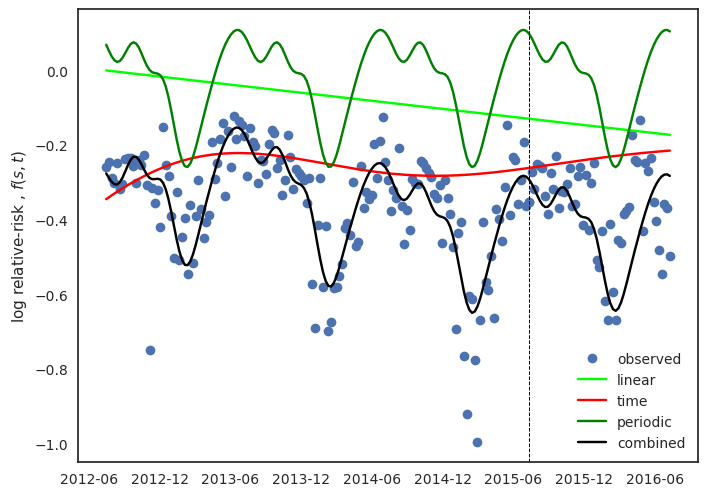
\includegraphics[width=0.5\textwidth]{citywide_var_decomp}
\end{figure}


 \subsection{Neighborhood Predictions}

 A neighborhood level model adds a spatial component to the existing temporal model.  New York City defines official Neighborhood Tabulation Areas (NTAs), which were used as the geographic areas of interest. The model was fit on the 29 official NTAs in the borough of Manhattan using 52 weeks of weekly pedestrian injury data. The spatial component was calculated from the distance between centroids for each NTA. \par


 \begin{figure}[h!]
   \caption{Manhattan's 29 neighborhoods, with red dots indicating the centroid used for calculating distance.}
   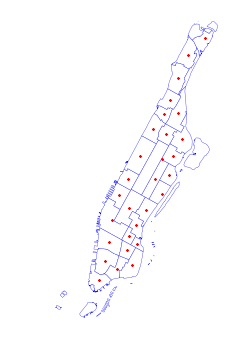
\includegraphics[width=0.5\textwidth]{mn_centroids}
 \end{figure}


Since the exponentiated latent function $exp(f(s,t))$ is directly interpretable as a measure of relative risk it can be used for direct comparisons between neighborhoods \par

 \begin{figure}[h!]
   \caption{Relative risk scores for Manhattan neighborhoods. Midtown is roughly twice as dangerous for pedestrians than Manhattan as a whole.}
   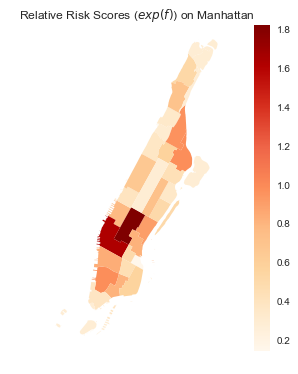
\includegraphics[width=0.5\textwidth]{mn_f_score_map}
 \end{figure}

A similar assessment of relative risk can be done across periods, A comparison between three Manhattan neighborhoods shows varying levels of latent risk while all three are subject to seasonality and periodicity.

\begin{figure}[h!]
  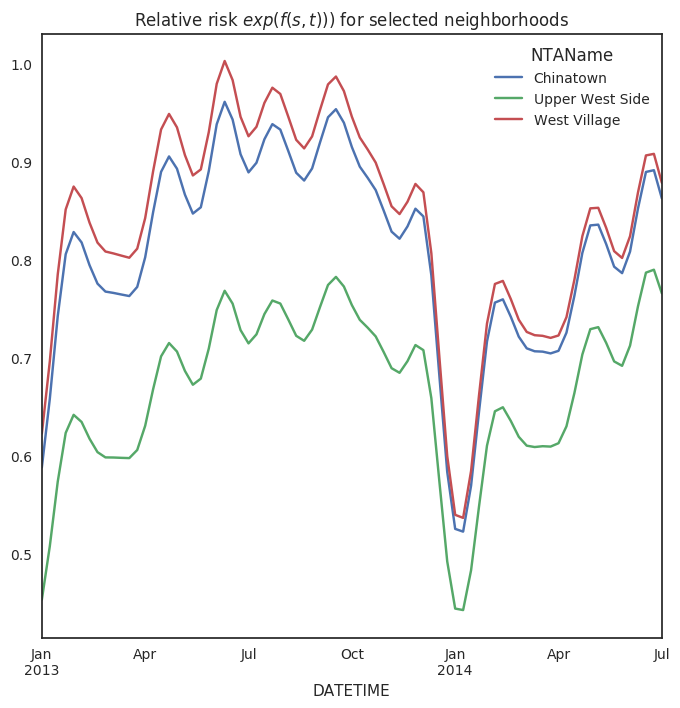
\includegraphics[width=0.5\textwidth]{MN_f_neighbs_example}
\end{figure}



\begin{table}[]
\centering
\caption{Neighborhood Reduction in Variance}
\label{variance_neighb}
\begin{tabular}{@{}lll@{}}
\toprule
                   & Reduction in Variance &  \\ \midrule
Time (RBF)         & 27.2\%                &  \\
Spatial (Matern32) & 22.3\%                &  \\
Periodic           & 2.0\%                 &  \\
Product            & 19.2\%                &  \\
Combined           & 64.6\%                &  \\ \bottomrule
\end{tabular}
\end{table}





\subsection{Short Term Forecasting}
